%%%%%%%%%%%%%%%%%%%%%%%%%%%%%%%%%%%%
% Slide options
%%%%%%%%%%%%%%%%%%%%%%%%%%%%%%%%%%%%

% Option 1: Slides with solutions

\documentclass[slidestop,compress,mathserif]{beamer}
\newcommand{\soln}[1]{\textit{#1}}
\newcommand{\solnGr}[1]{#1}

% Option 2: Handouts without solutions

%\documentclass[11pt,containsverbatim,handout]{beamer}
%\usepackage{pgfpages}
%\pgfpagesuselayout{4 on 1}[letterpaper,landscape,border shrink=5mm]
%\newcommand{\soln}[1]{ }
%\newcommand{\solnGr}{ }

%%%%%%%%%%%%%%%%%%%%%%%%%%%%%%%%%%%%
% Style
%%%%%%%%%%%%%%%%%%%%%%%%%%%%%%%%%%%%
\def\chp7@path{../../Chp 7}
\input{../../lec_style.tex}


%%%%%%%%%%%%%%%%%%%%%%%%%%%%%%%%%%%%
% Preamble
%%%%%%%%%%%%%%%%%%%%%%%%%%%%%%%%%%%%

\title[Lecture 29]{MA213: Lecture 30}
\subtitle{Module 4: Inference}
\author{OpenIntro Statistics, 4th Edition}
\institute{$\:$ \\ {\footnotesize Based on slides developed by Mine \c{C}etinkaya-Rundel of OpenIntro. \\
The slides may be copied, edited, and/or shared via the \webLink{http://creativecommons.org/licenses/by-sa/3.0/us/}{CC BY-SA license.} \\
Some images may be included under fair use guidelines (educational purposes).}}
\date{}


%%%%%%%%%%%%%%%%%%%%%%%%%%%%%%%%%%%%
% Begin document
%%%%%%%%%%%%%%%%%%%%%%%%%%%%%%%%%%%%

\begin{document}


%%%%%%%%%%%%%%%%%%%%%%%%%%%%%%%%%%%%
% Title page
%%%%%%%%%%%%%%%%%%%%%%%%%%%%%%%%%%%%

{
\addtocounter{framenumber}{-1} 
{\removepagenumbers 
\usebackgroundtemplate{
\includegraphics[width=\paperwidth]{../../OpenIntro_Grid_4_3-01.jpg}}
\begin{frame}

\hfill 
\includegraphics[width=20mm]{../../oiLogo_highres}

\titlepage

\end{frame}
}
}


%%%%%%%%%%%%%%%%%%%%%%%%%%%%%%%%%%%%
% Recap/Agenda 
%%%%%%%%%%%%%%%%%%%%%%%%%%%%%%%%%%%%
% TODO better formatting
\begin{frame}
    \frametitle{Module 4: Inference}
    \begin{itemize}
        \item \hl{Previously: }Comparing many means with ANOVA (Chapter 7.5)
        \item \hl{This time: }Issues with Hypothesis Testing 2: Multiple comparisons
        \item \hl{Reading: }Chapter 8.1 for next time
        \item \hl{Deadlines/Announcements: }
    \end{itemize}
    
\end{frame}

%%%%%%%%%%%%%%%%%%%%%%%%%%%%%%%%%%%%
% Learning objectives:
%%%%%%%%%%%%%%%%%%%%%%%%%%%%%%%%%%%%
\begin{frame}
    \frametitle{Learning Objectives}
    \begin{itemize}
        \item \textbf{M3, LO4: Explain Hypothesis Testing and Its Limitations:} Discuss the use cases and potential issues with hypothesis testing, including the interpretation of results.
        \item \textbf{M3, LO6: Distinguish Statistical vs. Practical Significance:} Differentiate between statistical significance and practical significance, and explain the implications of each.
        \item \textbf{M4: LO8: Conduct and Interpret ANOVA:} Assess whether conditions for an ANOVA are met, and if so, design, execute, and interpret the test to compare sample means across several groups.
    \end{itemize}
\end{frame}

%%%%%%%%%%%%%%%%%%%%%%%%%%%%%%%%%%%%
% Sections
%%%%%%%%%%%%%%%%%%%%%%%%%%%%%%%%%%%%

%%%%%%%%%%%%%%%%%%%%%%%%%%%%%%%%%%%

\section{Review}

\begin{frame}
\frametitle{}

\begin{center}
\includegraphics[width=0.5\textwidth]{\chp7@path/7-5_anova/figures/aldrin/wolf}
\end{center}

{\small
\begin{itemize}

\item  The Wolf River in Tennessee flows past an abandoned site once used by the pesticide industry for dumping wastes, including chlordane (pesticide), aldrin, and dieldrin (both insecticides).

% \pause

\item These highly toxic organic compounds can cause various cancers and birth defects.

% \pause

\item The standard methods to test whether these substances are present in a river is to take samples at six-tenths depth. 

% \pause

\item But since these compounds are denser than water and their molecules tend to stick to particles of sediment, they are more likely to be found in higher concentrations near the bottom than near mid-depth.

\end{itemize}
}

\end{frame}

%%%%%%%%%%%%%%%%%%%%%%%%%%%%%%%%%%%

\begin{frame}
\frametitle{ANOVA}

ANOVA is used to assess whether the mean of the outcome variable is different for different levels of a categorical variable.

% \pause

\begin{itemize}
\item[] \mathhl{H_0:} The mean outcome is the same across all categories, 
\[\mu_1 = \mu_2 = \cdots = \mu_k, \]
where $\mu_i$ represents the mean of the outcome for observations in category $i$.
\item[]
\item[] \mathhl{H_A:} At least one mean is different than others.
\end{itemize}

\end{frame}

%%%%%%%%%%%%%%%%%%%%%%%%%%%%%%%%%%

\begin{frame}
\frametitle{Conditions}

\begin{enumerate}

\item The observations should be independent within and between groups

\begin{itemize}
\item If the data are a simple random sample from less than 10\% of the population, this condition is satisfied.
\item Carefully consider whether the data may be independent (e.g. no pairing). 
\item Always important, but sometimes difficult to check.
\end{itemize}

% \pause

\item The observations within each group should be nearly normal.

\begin{itemize}
\item Especially important when the sample sizes are small.
\end{itemize}

\dq{How do we check for normality?}

% \pause

\item The variability across the groups should be about equal.

\begin{itemize}
\item Especially important when the sample sizes differ between groups.
\end{itemize}

\dq{How can we check this condition?}

\end{enumerate}

\end{frame}

%%%%%%%%%%%%%%%%%%%%%%%%%%%%%%%%%%%

\begin{frame}
\frametitle{}

\vspace{-0.25cm}

{\footnotesize
\begin{center}
\begin{tabular}{ll rrr>{\columncolor[gray]{.6}[.5\tabcolsep]}rr}
\hline
 			& 			& Df 	& Sum Sq	& Mean Sq 	& F value 	& Pr($>$F) \\ 
\hline
(\hl{G}roup) 	& depth 		& 2 	& 16.96	& 8.48 		& \orange{6.14} 	& 0.0063 \\ 
(\hl{E}rror) 	& Residuals 	& 27 	& 37.33 	& 1.38 		&  		&  \\ 
\hline
	 		& \hl{T}otal	& 29	& 54.29 \\
\end{tabular}
\end{center}
}

\formula{Test statistic, F value}
{
As we discussed before, the F statistic is the ratio of the between group and within group variability.
\[ F = \frac{MSG}{MSE} \]
}

% \pause

\[ F = \frac{8.48}{1.38} = 6.14 \]

\end{frame}

%%%%%%%%%%%%%%%%%%%%%%%%%%%%%%%%%%%
\begin{frame}
% \frametitle{p-value in ANOVA}

\vspace{-0.25cm}

{\footnotesize
\begin{center}
\begin{tabular}{ll rrr>{\columncolor[gray]{.6}[.5\tabcolsep]}rr}
\hline
                & 			& Df 	& Sum Sq	& Mean Sq 	& F value 	& Pr($>$F) \\ 
\hline
(\hl{G}roup) 	& depth 		& 2 	& 16.96	& 8.48 		& \orange{6.14} 	& 0.0063 \\ 
(\hl{E}rror) 	& Residuals 	& 27 	& 37.33 	& 1.38 		&  		&  \\ 
\hline
                & \hl{T}otal	& 29	& 54.29 \\
\end{tabular}
\end{center}
}

\formula{p-value}
{
p-value is the probability of at least as large a ratio between the ``between group" and ``within group" variability, if in fact the means of all groups are equal. It's calculated as the area under the F curve, with degrees of freedom $df_G$ and $df_E$, above the observed F statistic.
}

% \pause

\includegraphics[width=0.9\textwidth]{\chp7@path/7-5_anova/figures/aldrin/f}

\end{frame}

%%%%%%%%%%%%%%%%%%%%%%%%%%%%%%%%%%%

\subsection{Multiple comparisons \& Type 1 error rate}

%%%%%%%%%%%%%%%%%%%%%%%%%%%%%%%%%%%

\begin{frame}
\frametitle{Which means differ?}

\begin{itemize}

\item Earlier we concluded that at least one pair of means differ. The natural question that follows is ``which ones?"

\pause

\item We can do two sample $t$ tests for differences in each possible pair of groups.

\pause

\end{itemize}

\dq{Can you see any pitfalls with this approach?}

% \pause

% \begin{itemize}

% \item When we run too many tests, the Type 1 Error rate increases.

% \item This issue is resolved by using a modified significance level.

% \end{itemize}

\end{frame}

%%%%%%%%%%%%%%%%%%%%%%%%%%%%%%%%%%%

\begin{frame}
\begin{center}
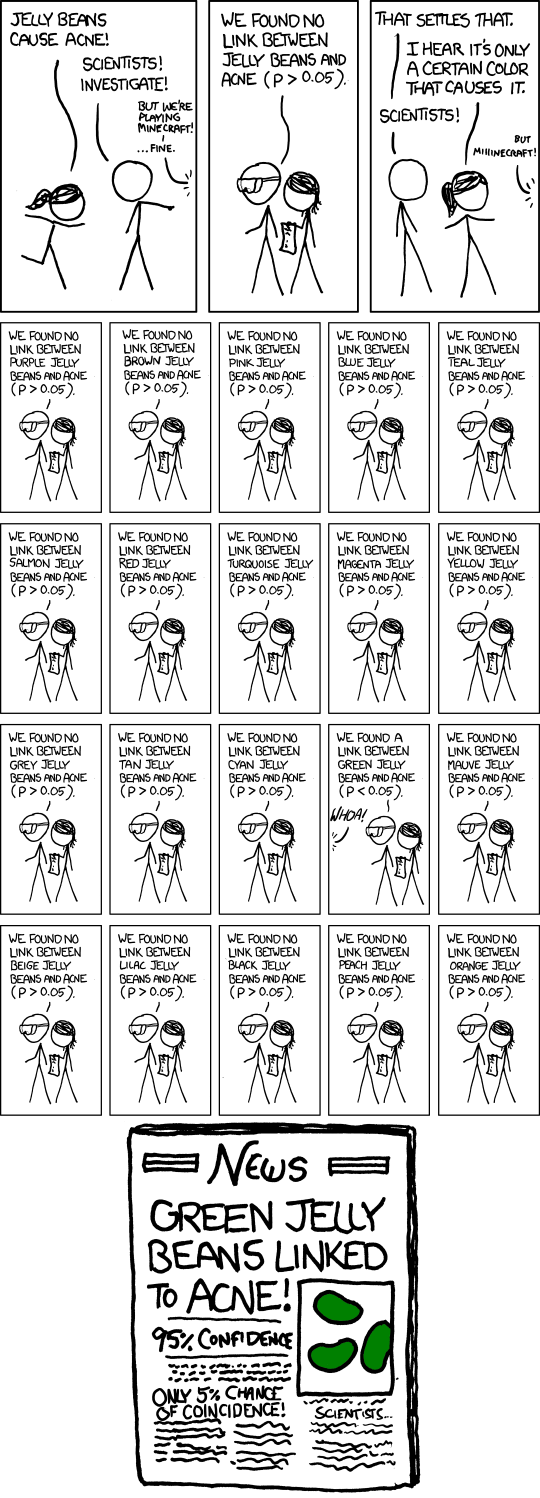
\includegraphics[width=0.9\textwidth]{xkcd_significance.png}
\end{center}
\end{frame}

%%%%%%%%%%%%%%%%%%%%%%%%%%%%%%%%%%%

\begin{frame}
\begin{center}
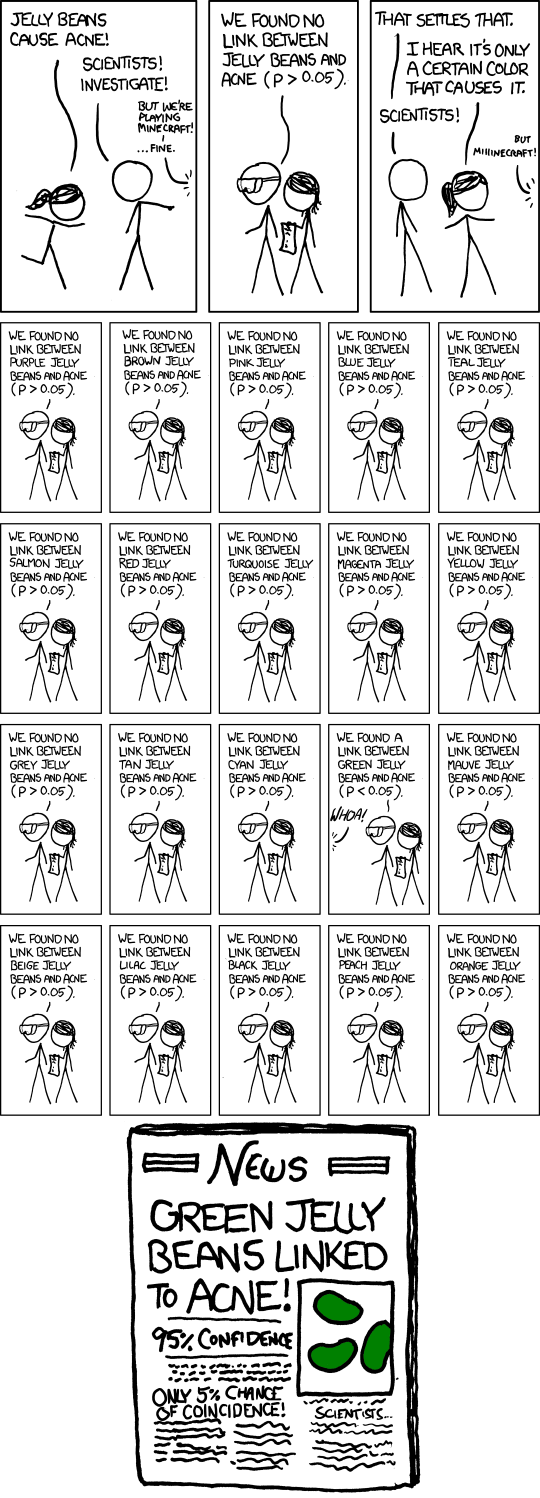
\includegraphics[height=0.95\textheight]{xkcd_significance.png}
\end{center}

\footnotesize https://imgs.xkcd.com/comics/significant.png
\end{frame}

%%%%%%%%%%%%%%%%%%%%%%%%%%%%%%%%%%%

\section{Edfinity Quiz: Multiple Comparisons}

%%%%%%%%%%%%%%%%%%%%%%%%%%%%%%%%%%%

\begin{frame}
\frametitle{Multiple comparisons and Type I Error Rate}
If $\alpha=0.05$:
\begin{itemize}
\item \dq{What is the chance that I get a type I error when doing 1 test?} \soln{\only<2-5>{ 0.05 (5\%) } }
\item \dq{How many Type I errors would I expect if I did 20 independent tests with no true effects?} \soln{\only<3-5>{ 1 (20 x 0.05) } }
\item \dq{What is the probability of at least one Type I error if I do 20 independent tests with no true effects?} \soln{\only<4-5>{ $1 - (1 - 0.05)^{20} \approx 0.64$ (64\%) } }
\item \dq{What should I do to alpha if I want to control the probability of at least one Type I error?} \soln{\only<5>{ make it smaller } }
\end{itemize}


\end{frame}

%%%%%%%%%%%%%%%%%%%%%%%%%%%%%%%%%%%

\begin{frame}
\frametitle{Multiple comparisons}

\begin{itemize}

\item The scenario of testing many pairs of groups is called \hl{multiple comparisons}.

\pause

\item The \hl{Bonferroni correction} suggests that a more \orange{stringent} significance level is more appropriate for these tests:

\[ \alpha^\star = \alpha / K \]

where $K$ is the number of comparisons being considered.

\pause

\item If there are $k$ groups, then usually all possible pairs are compared and $K = \frac{k (k - 1)}{2}$.

\pause

\item This correction controls the \hl{familywise error rate} (FWER), which is the probability of making at least one Type I error among all the tests.

\end{itemize}

\end{frame}

%%%%%%%%%%%%%%%%%%%%%%%%%%%%%%%%%%%

\begin{frame}
\frametitle{Determining the modified $\alpha$}

\pq{In the aldrin data set depth has 3 levels: bottom, mid-depth, and surface. If $\alpha = 0.05$, what should be the modified significance level for two sample $t$ tests for determining which pairs of groups have significantly different means?}

\begin{enumerate}[(a)]
\item $\alpha^* = 0.05$
\item $\alpha^* = 0.05 / 2 = 0.025$
\solnMult{$\alpha^* = 0.05 / 3 = 0.0167$}
\item $\alpha^* = 0.05 / 6 = 0.0083$
\end{enumerate}

\end{frame}

%%%%%%%%%%%%%%%%%%%%%%%%%%%%%%%%%%%

\begin{frame}
\frametitle{Which means differ?}

\pq{Based on the box plots below, which means would you expect to be significantly different?}

\twocol{0.6}{0.4}{
\includegraphics[width=\textwidth]{\chp7@path/7-5_anova/figures/aldrin/homo}
}
{
\begin{enumerate}[(a)]
\item bottom \& surface
\item bottom \& mid-depth
\item mid-depth \& surface
\item bottom \& mid-depth; mid-depth \& surface
\item bottom \& mid-depth; bottom \& surface; mid-depth \& surface
\end{enumerate}
}

\end{frame}

%%%%%%%%%%%%%%%%%%%%%%%%%%%%%%%%%%

\begin{frame}
\frametitle{Which means differ? (cont.)}

If the ANOVA assumption of equal variability across groups is satisfied, we can use the data from all groups to estimate variability:
    
\begin{itemize}

\item Estimate any within-group standard deviation with $\sqrt{MSE}$, which is $s_{pooled}$

\item Use the error degrees of freedom, $n - k$, for $t$-distributions

\end{itemize}

\formula{Difference in two means: after ANOVA}{
\[ SE = \sqrt{  \frac{\sigma_1^2}{n_1} + \frac{\sigma_2^2}{n_2} } \approx \sqrt{ \frac{MSE}{n_1} + \frac{MSE}{n_2} } \]
}

\end{frame}

%%%%%%%%%%%%%%%%%%%%%%%%%%%%%%%%%%

\begin{frame}
\frametitle{}

\dq{Is there a difference between the  average aldrin concentration at the bottom and at mid depth?}

\twocol{0.4}{0.7}{
{\scriptsize
\begin{center}
\begin{tabular}{l | c c c}
        & n	& mean	& sd		\\
\hline
bottom	& 10	& \orange{6.04}	& 1.58 \\
middepth& 10	& \orange{5.05}	& 1.10 \\
surface	& 10	& 4.2 	& 0.66 \\
\hline
overall	& 30	& 5.1		& 1.37
\end{tabular}
\end{center}
}
}
{
{\scriptsize
\begin{center}
\begin{tabular}{l rrrrr}
\hline
                & Df 	& Sum Sq	& Mean Sq 	& F value 	& Pr($>$F) \\ 
\hline
depth 		& 2 	& 16.96 	& 8.48 		& 6.13 	& 0.0063 \\ 
Residuals 	& \orange{27} 	& 37.33 	& \orange{1.38} 		&  		&  \\ 
\hline
Total			& 29	& 54.29 \\
\end{tabular}
\end{center}
}
}

\begin{eqnarray*}
T_{df_E} &=& \frac{(\bar{x}_{bottom} - \bar{x}_{middepth})}{\sqrt{ \frac{MSE}{n_{bottom}} + \frac{MSE}{n_{middepth}} }} \\ 
\pause
T_{27} &=& \frac{( 6.04 - 5.05 )}{\sqrt{ \frac{1.38}{10} + \frac{1.38}{10} }} = \frac{0.99}{0.53}  =1.87 \\
\pause
0.05 &<& p-value < 0.10 \qquad \text{{\footnotesize (two-sided)}} \\
\pause
\alpha^\star &=& 0.05 / 3 = 0.0167
\end{eqnarray*}

\pause
{\small Fail to reject $H_0$, data do not provide convincing evidence of a difference between average aldrin concentrations at bottom and mid depth.}

\end{frame}

%%%%%%%%%%%%%%%%%%%%%%%%%%%%%%%%%%

\begin{frame}
\frametitle{}

\app{Pairwise comparisons}{Is there a difference between the  average aldrin concentration at the bottom and at surface?}

\pause

\soln{
\begin{eqnarray*}
T_{df_E} &=& \frac{(\bar{x}_{bottom} - \bar{x}_{surface})}{\sqrt{ \frac{MSE}{n_{bottom}} + \frac{MSE}{n_{surface}} }} \\ 
\pause
T_{27} &=& \frac{( 6.04 - 4.2 )}{\sqrt{ \frac{1.38}{10} + \frac{1.38}{10} }} = \frac{1.84}{0.53}  =3.47 \\
\pause
p-value = 0.0018 \qquad \text{{\footnotesize (two-sided)}} \\
\pause
\alpha^\star &=& 0.05 / 3 = 0.0167
\end{eqnarray*}
\pause
{\small Reject $H_0$, the data provide convincing evidence of a difference between the average aldrin concentrations at bottom and surface.}
}

\end{frame}

%%%%%%%%%%%%%%%%%%%%%%%%%%%%%%%%%%

\begin{frame}
\frametitle{P-Hacking}

What if we looked at the data and decided to run only the bottom vs. surface test because we saw that those box plots looked the most different?

Since we only ran one test, we could use $\alpha = 0.05$ instead of the Bonferroni corrected $\alpha^\star = 0.0167$, right???

\pause

This is called \hl{p-hacking} or \hl{data dredging/snooping/fishing}, and it inflates the Type I error rate!

It is unethical, because it misleads others into thinking there is stronger evidence against the null hypothesis than there really is.

\pause

To avoid p-hacking, we should decide on the analyses to be done before looking at the data (\hl{preregistration}).
\end{frame}

%%%%%%%%%%%%%%%%%%%%%%%%%%%%%%%%%%

\begin{frame}
\frametitle{The Garden of Forking Paths}

Multiple comparisons can be \hl{unintentional}. Consider all of the decisions that can be made during data collection, analysis, and reporting, e.g.:
\begin{itemize}
\item Outlier removal: after plotting data, there are some extreme values. Should we remove outliers or not?
\item Choice of statistics of interest: compare means vs medians?
\item Transformations: maybe transform the response (log / square root) if skewed.
\item Subgroup analysis: split by gender or by study hours (above vs below median) and test separately.
\end{itemize}

\hl{Over time, these choices can lead to an increased Type I error rate, even if each individual test is done at the nominal significance level.}

\end{frame}

%%%%%%%%%%%%%%%%%%%%%%%%%%%%%%%%%%

\begin{frame}
\frametitle{The Garden of Forking Paths}
\begin{center}
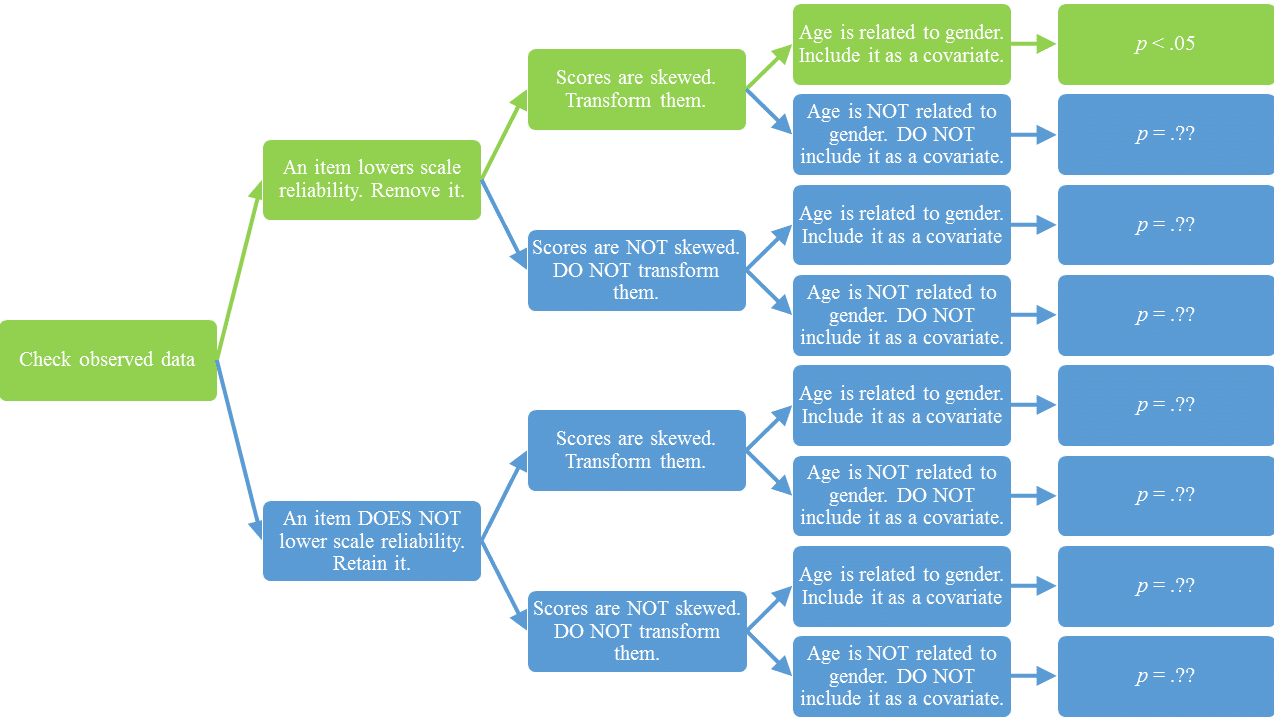
\includegraphics[width=0.95\textwidth]{Rubin_forkingPaths.png}
\end{center}
\footnotesize Mark Rubin https://doi.org/10.1037/gpr0000135
\end{frame}
%%%%%%%%%%%%%%%%%%%%%%%%%%%%%%%%%%

\begin{frame}
\frametitle{Recall: Beauty and Sex Ratios Case Study}

\begin{itemize}
    \item \textbf{Claim:} Attractive people are more likely to have female children.
    \item Survey respondents rated for attractiveness; sex of first child recorded.
    \item Reported difference: Most attractive (rating 5) had 56\% girls, others (ratings 1-4) had 48\% girls.
    \item Statistical test found a significant difference ($p$-value $=0.015$).
    \item Realistic effect sizes for sex ratios are much smaller (about 1\%).
\end{itemize}
\end{frame}

\begin{frame}
\frametitle{Design Choices and Inflated Type I Error Rate}

\begin{itemize}
    \item Many decisions in study design and analysis can unintentionally increase the chance of false positives:
    \begin{itemize}
        \item How to group attractiveness ratings (e.g., 5 vs 1-4, or other splits)?
        \item Whether to include/exclude certain respondents or outliers.
        \item Choice of outcome variable (first child, all children, etc.).
        \item Selection of statistical tests and transformations.
        \item Subgroup analyses (e.g., by age, gender, etc.).
    \end{itemize}
    \item Each choice can be seen as a ``fork'' in the analysis path, increasing the Type I error rate.
    \item Without preregistration or correction for multiple comparisons, reported $p$-values may be misleading.
\end{itemize}
\end{frame}

%%%%%%%%%%%%%%%%%%%%%%%%%%%%%%%%%%%

\begin{frame}
\frametitle{Best Practices for Statistical Analysis}
\begin{itemize}
    \item Avoid hypothesis testing when inappropriate
    \item Preregister analysis plans to prevent data dredging
    \item Report effect sizes and confidence intervals alongside p-values
    \item Use data splitting for exploratory work to validate findings
\end{itemize}
\end{frame}

%%%%%%%%%%%%%%%%%%%%%%%%%%%%%%%%%%%


\begin{frame}
\begin{center}
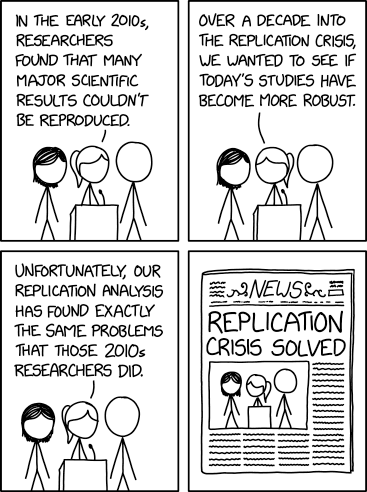
\includegraphics[height=0.95\textheight]{xkcd_replication_crisis.png}
\end{center}

\footnotesize https://imgs.xkcd.com/comics/replication\_crisis.png
\end{frame}

%%%%%%%%%%%%%%%%%%%%%%%%%%%%%%%%%%%

%%%%%%%%%%%%%%%%%%%%%%%%%%%%%%%%%%    


%%%%%%%%%%%%%%%%%%%%%%%%%%%%%%%%%%%%
% End document
%%%%%%%%%%%%%%%%%%%%%%%%%%%%%%%%%%%%

\end{document}